\section{Achados da Pesquisa}

Para o estudo de caso, os dados obtidos nas entrevistas s�o apresentados de
acordo com a divis�o de grupo, cada grupo � apresentado e analisado
individualmente, permitindo assim, maior entendimento dos resultados obitidos.

\begin{table}
\caption{Dados Diretoria}
\begin{tabularx}{\textwidth}{|p{6cm}|X|X|X|X|X|X|}
\hline
\theadone \hline
\multirow{3}{\tlen}{\PS} & a & 0 & 0 & 0 & 0 & 2 \\ \cline{2-7}
                         & b & 0 & 0 & 0 & 0 & 2 \\ \cline{2-7}
                         & c & 0 & 0 & 1 & 0 & 1 \\ \hline

\multirow{5}{\tlen}{\SO} & a & 0 & 0 & 0 & 1 & 1 \\ \cline{2-7}
                         & b & 0 & 0 & 1 & 1 & 0 \\ \cline{2-7}
                         & c & 0 & 0 & 2 & 0 & 0 \\ \cline{2-7}
                         & d & 0 & 0 & 0 & 2 & 0 \\ \cline{2-7}
                         & e & 0 & 0 & 0 & 1 & 1 \\ \hline

\multirow{2}{\tlen}{\CI} & a & 0 & 0 & 0 & 0 & 2 \\ \cline{2-7}
                         & b & 0 & 0 & 1 & 1 & 0 \\ \hline

\multirow{4}{\tlen}{\SP} & a & 0 & 0 & 0 & 1 & 1 \\ \cline{2-7}
                         & b & 0 & 0 & 0 & 0 & 2 \\ \cline{2-7}
                         & c & 0 & 0 & 0 & 1 & 1 \\ \cline{2-7}
                         & d & 0 & 0 & 1 & 1 & 0 \\ \hline

\multirow{4}{\tlen}{\SF} & a & 0 & 0 & 0 & 0 & 2 \\ \cline{2-7}
                         & b & 0 & 0 & 0 & 2 & 0 \\ \cline{2-7}
                         & c & 0 & 0 & 0 & 1 & 1 \\ \cline{2-7}
                         & d & 0 & 0 & 0 & 1 & 1 \\ \hline

\multirow{8}{\tlen}{\GO} & a & 0 & 0 & 0 & 1 & 1 \\ \cline{2-7}
                         & b & 0 & 0 & 0 & 2 & 0 \\ \cline{2-7}
                         & c & 0 & 0 & 0 & 2 & 0 \\ \cline{2-7}
                         & d & 0 & 0 & 0 & 2 & 0 \\ \cline{2-7}
                         & e & 0 & 0 & 1 & 1 & 0 \\ \cline{2-7}
                         & f & 0 & 0 & 0 & 1 & 1 \\ \cline{2-7}
                         & g & 0 & 0 & 0 & 2 & 0 \\ \cline{2-7}
                         & h & 0 & 0 & 0 & 1 & 1 \\ \hline

\multirow{6}{\tlen}{\CA} & a & 0 & 0 & 0 & 1 & 1 \\ \cline{2-7}
                         & b & 0 & 0 & 0 & 1 & 1 \\ \cline{2-7}
                         & c & 0 & 0 & 0 & 1 & 1 \\ \cline{2-7}
                         & d & 0 & 0 & 0 & 1 & 1 \\ \cline{2-7}
                         & e & 0 & 0 & 0 & 1 & 1 \\ \cline{2-7}
                         & f & 0 & 0 & 0 & 1 & 1 \\ \hline

\multirow{3}{\tlen}{\DS} & a & 0 & 0 & 0 & 2 & 0 \\ \cline{2-7}
                         & b & 0 & 0 & 0 & 1 & 1 \\ \cline{2-7}
                         & c & 0 & 0 & 0 & 1 & 1 \\ \hline

\multirow{2}{\tlen}{\GN} & a & 0 & 0 & 0 & 2 & 0 \\ \cline{2-7}
                         & b & 0 & 0 & 0 & 1 & 1 \\ \hline

\multirow{3}{\tlen}{\CO} & a & 0 & 0 & 0 & 2 & 0 \\ \cline{2-7}
                         & b & 0 & 0 & 0 & 2 & 0 \\ \cline{2-7}
                         & c & 0 & 0 & 0 & 2 & 0 \\ \hline

\multirow{7}{\tlen}{\GC} & a & 0 & 0 & 0 & 0 & 2 \\ \cline{2-7}
                         & b & 0 & 0 & 0 & 0 & 2 \\ \cline{2-7}
                         & c & 0 & 0 & 0 & 1 & 1 \\ \cline{2-7}
                         & d & 0 & 0 & 1 & 1 & 0 \\ \cline{2-7}
                         & e & 0 & 0 & 1 & 0 & 1 \\ \cline{2-7}
                         & f & 0 & 0 & 0 & 1 & 1 \\ \cline{2-7}
                         & g & 0 & 0 & 0 & 2 & 0 \\ \hline

\end{tabularx}
\end{table}

\begin{table}[H]\footnotesize
\caption{Dados Gerentes}
\begin{tabularx}{\textwidth}{|p{6cm}|X|X|X|X|X|X|}
\hline
\theadone \hline
\multirow{3}{\tlen}{\PS} & a & 0 & 0 & 0 & 2 & 5 \\ \cline{2-7}
                         & b & 0 & 0 & 0 & 3 & 4 \\ \cline{2-7}
                         & c & 0 & 0 & 1 & 2 & 4 \\ \hline

\multirow{5}{\tlen}{\SO} & a & 0 & 0 & 0 & 2 & 5 \\ \cline{2-7}
                         & b & 1 & 0 & 0 & 3 & 3 \\ \cline{2-7}
                         & c & 0 & 0 & 1 & 4 & 2 \\ \cline{2-7}
                         & d & 0 & 0 & 2 & 1 & 4 \\ \cline{2-7}
                         & e & 0 & 0 & 1 & 2 & 4 \\ \hline

\multirow{2}{\tlen}{\CI} & a & 0 & 0 & 2 & 0 & 5 \\ \cline{2-7}
                         & b & 0 & 0 & 0 & 2 & 5 \\ \hline

\multirow{4}{\tlen}{\SP} & a & 0 & 0 & 0 & 2 & 5 \\ \cline{2-7}
                         & b & 0 & 0 & 0 & 3 & 4 \\ \cline{2-7}
                         & c & 0 & 0 & 1 & 4 & 2 \\ \cline{2-7}
                         & d & 0 & 0 & 0 & 5 & 2 \\ \hline

\multirow{4}{\tlen}{\SF} & a & 0 & 0 & 2 & 4 & 1 \\ \cline{2-7}
                         & b & 0 & 0 & 1 & 4 & 2 \\ \cline{2-7}
                         & c & 1 & 0 & 0 & 2 & 4 \\ \cline{2-7}
                         & d & 1 & 0 & 0 & 2 & 4 \\ \hline

\multirow{8}{\tlen}{\GO} & a & 0 & 0 & 0 & 3 & 4 \\ \cline{2-7}
                         & b & 1 & 0 & 0 & 3 & 3 \\ \cline{2-7}
                         & c & 1 & 0 & 0 & 4 & 2 \\ \cline{2-7}
                         & d & 1 & 0 & 1 & 2 & 3 \\ \cline{2-7}
                         & e & 0 & 0 & 4 & 0 & 3 \\ \cline{2-7}
                         & f & 0 & 0 & 0 & 3 & 4 \\ \cline{2-7}
                         & g & 0 & 0 & 1 & 4 & 2 \\ \cline{2-7}
                         & h & 0 & 0 & 0 & 3 & 4 \\ \hline

\multirow{6}{\tlen}{\CA} & a & 0 & 0 & 0 & 1 & 6 \\ \cline{2-7}
                         & b & 0 & 0 & 1 & 2 & 4 \\ \cline{2-7}
                         & c & 0 & 0 & 1 & 0 & 6 \\ \cline{2-7}
                         & d & 0 & 0 & 0 & 1 & 6 \\ \cline{2-7}
                         & e & 0 & 0 & 1 & 0 & 6 \\ \cline{2-7}
                         & f & 0 & 0 & 1 & 1 & 5 \\ \hline

\multirow{3}{\tlen}{\DS} & a & 0 & 0 & 0 & 2 & 5 \\ \cline{2-7}
                         & b & 0 & 0 & 1 & 1 & 5 \\ \cline{2-7}
                         & c & 0 & 0 & 0 & 1 & 6 \\ \hline

\multirow{2}{\tlen}{\GN} & a & 0 & 0 & 0 & 3 & 4 \\ \cline{2-7}
                         & b & 0 & 0 & 0 & 3 & 4 \\ \hline

\multirow{3}{\tlen}{\CO} & a & 1 & 0 & 0 & 2 & 4 \\ \cline{2-7}
                         & b & 0 & 0 & 0 & 4 & 3 \\ \cline{2-7}
                         & c & 1 & 0 & 0 & 3 & 3 \\ \hline

\multirow{7}{\tlen}{\GC} & a & 0 & 0 & 0 & 4 & 3 \\ \cline{2-7}
                         & b & 0 & 0 & 2 & 3 & 2 \\ \cline{2-7}
                         & c & 0 & 0 & 1 & 4 & 3 \\ \cline{2-7}
                         & d & 1 & 0 & 2 & 2 & 3 \\ \cline{2-7}
                         & e & 0 & 0 & 2 & 3 & 3 \\ \cline{2-7}
                         & f & 0 & 0 & 0 & 4 & 3 \\ \cline{2-7}
                         & g & 0 & 0 & 0 & 4 & 3 \\ \hline

\end{tabularx}
\end{table}

\begin{table}
\caption{Dados Efetivos}
\begin{tabularx}{\textwidth}{|p{6cm}|X|X|X|X|X|X|}
\hline
\theadone \hline
\multirow{3}{\tlen}{\PS} & a & 0 & 0 & 0 & 2 & 9 \\ \cline{2-7}
                         & b & 0 & 0 & 0 & 0 & 11 \\ \cline{2-7}
                         & c & 0 & 0 & 0 & 1 & 10 \\ \hline

\multirow{5}{\tlen}{\SO} & a & 1 & 0 & 0 & 0 & 10 \\ \cline{2-7}
                         & b & 2 & 1 & 0 & 3 & 5 \\ \cline{2-7}
                         & c & 1 & 0 & 1 & 1 & 8 \\ \cline{2-7}
                         & d & 1 & 0 & 1 & 0 & 9 \\ \cline{2-7}
                         & e & 1 & 0 & 1 & 0 & 9 \\ \hline

\multirow{2}{\tlen}{\CI} & a & 0 & 0 & 0 & 4 & 7 \\ \cline{2-7}
                         & b & 0 & 0 & 0 & 4 & 7 \\ \hline

\multirow{4}{\tlen}{\SP} & a & 0 & 0 & 1 & 3 & 7 \\ \cline{2-7}
                         & b & 0 & 0 & 1 & 2 & 8 \\ \cline{2-7}
                         & c & 0 & 0 & 1 & 1 & 9 \\ \cline{2-7}
                         & d & 0 & 0 & 1 & 4 & 6 \\ \hline

\multirow{4}{\tlen}{\SF} & a & 0 & 0 & 3 & 2 & 6 \\ \cline{2-7}
                         & b & 0 & 0 & 1 & 2 & 8 \\ \cline{2-7}
                         & c & 1 & 0 & 0 & 2 & 8 \\ \cline{2-7}
                         & d & 2 & 1 & 0 & 3 & 5 \\ \hline

\multirow{8}{\tlen}{\GO} & a & 2 & 1 & 1 & 1 & 6 \\ \cline{2-7}
                         & b & 1 & 0 & 0 & 3 & 7 \\ \cline{2-7}
                         & c & 1 & 0 & 1 & 2 & 7 \\ \cline{2-7}
                         & d & 1 & 0 & 0 & 3 & 7 \\ \cline{2-7}
                         & e & 1 & 0 & 1 & 1 & 8 \\ \cline{2-7}
                         & f & 1 & 0 & 1 & 0 & 9 \\ \cline{2-7}
                         & g & 1 & 0 & 1 & 0 & 9 \\ \cline{2-7}
                         & h & 1 & 0 & 1 & 1 & 8 \\ \hline

\multirow{6}{\tlen}{\CA} & a & 0 & 0 & 0 & 2 & 9 \\ \cline{2-7}
                         & b & 0 & 0 & 1 & 2 & 8 \\ \cline{2-7}
                         & c & 0 & 0 & 1 & 1 & 9 \\ \cline{2-7}
                         & d & 0 & 0 & 1 & 2 & 8 \\ \cline{2-7}
                         & e & 0 & 1 & 1 & 2 & 7 \\ \cline{2-7}
                         & f & 0 & 0 & 2 & 1 & 8 \\ \hline

\multirow{3}{\tlen}{\DS} & a & 1 & 0 & 1 & 0 & 9 \\ \cline{2-7}
                         & b & 1 & 0 & 0 & 3 & 7 \\ \cline{2-7}
                         & c & 1 & 0 & 1 & 2 & 7 \\ \hline

\multirow{2}{\tlen}{\GN} & a & 0 & 0 & 0 & 3 & 8 \\ \cline{2-7}
                         & b & 1 & 1 & 2 & 2 & 5 \\ \hline

\multirow{3}{\tlen}{\CO} & a & 1 & 0 & 0 & 2 & 8 \\ \cline{2-7}
                         & b & 1 & 0 & 0 & 3 & 7 \\ \cline{2-7}
                         & c & 1 & 0 & 0 & 3 & 7 \\ \hline

\multirow{7}{\tlen}{\GC} & a & 1 & 1 & 0 & 2 & 7 \\ \cline{2-7}
                         & b & 0 & 0 & 0 & 1 & 10 \\ \cline{2-7}
                         & c & 0 & 0 & 0 & 2 & 9 \\ \cline{2-7}
                         & d & 0 & 0 & 2 & 1 & 8 \\ \cline{2-7}
                         & e & 0 & 0 & 1 & 1 & 9 \\ \cline{2-7}
                         & f & 0 & 0 & 1 & 2 & 8 \\ \cline{2-7}
                         & g & 0 & 0 & 1 & 1 & 9 \\ \hline

\end{tabularx}
\end{table}

\begin{table}
\caption{Dados Terceiros} %
\begin{tabularx}{\textwidth}{|p{6cm}|X|X|X|X|X|X|}
\hline
\theadone \hline
\multirow{3}{\tlen}{\PS} & a & 0 & 0 & 0 & 0 & 8 \\ \cline{2-7}
                         & b & 0 & 0 & 0 & 2 & 6 \\ \cline{2-7}
                         & c & 0 & 0 & 0 & 2 & 6 \\ \hline

\multirow{5}{\tlen}{\SO} & a & 0 & 1 & 0 & 1 & 6 \\ \cline{2-7}
                         & b & 1 & 0 & 0 & 2 & 5 \\ \cline{2-7}
                         & c & 0 & 0 & 0 & 2 & 6 \\ \cline{2-7}
                         & d & 1 & 0 & 1 & 1 & 5 \\ \cline{2-7}
                         & e & 0 & 1 & 0 & 2 & 5 \\ \hline

\multirow{2}{\tlen}{\CI} & a & 0 & 0 & 1 & 2 & 5 \\ \cline{2-7}
                         & b & 0 & 0 & 2 & 2 & 4 \\ \hline

\multirow{4}{\tlen}{\SP} & a & 0 & 0 & 0 & 2 & 6 \\ \cline{2-7}
                         & b & 0 & 0 & 0 & 2 & 6 \\ \cline{2-7}
                         & c & 0 & 0 & 1 & 1 & 6 \\ \cline{2-7}
                         & d & 0 & 0 & 1 & 2 & 5 \\ \hline

\multirow{4}{\tlen}{\SF} & a & 0 & 0 & 1 & 2 & 5 \\ \cline{2-7}
                         & b & 0 & 0 & 0 & 2 & 6 \\ \cline{2-7}
                         & c & 0 & 0 & 0 & 1 & 7 \\ \cline{2-7}
                         & d & 0 & 0 & 0 & 1 & 7 \\ \hline

\multirow{8}{\tlen}{\GO} & a & 1 & 0 & 0 & 2 & 5 \\ \cline{2-7}
                         & b & 1 & 0 & 0 & 2 & 5 \\ \cline{2-7}
                         & c & 1 & 0 & 0 & 3 & 4 \\ \cline{2-7}
                         & d & 1 & 0 & 0 & 1 & 6 \\ \cline{2-7}
                         & e & 1 & 0 & 0 & 1 & 6 \\ \cline{2-7}
                         & f & 1 & 0 & 0 & 2 & 5 \\ \cline{2-7}
                         & g & 1 & 0 & 0 & 2 & 5 \\ \cline{2-7}
                         & h & 1 & 0 & 0 & 2 & 5 \\ \hline

\multirow{6}{\tlen}{\CA} & a & 0 & 0 & 0 & 2 & 6 \\ \cline{2-7}
                         & b & 0 & 0 & 0 & 1 & 7 \\ \cline{2-7}
                         & c & 0 & 0 & 0 & 2 & 6 \\ \cline{2-7}
                         & d & 0 & 0 & 0 & 2 & 6 \\ \cline{2-7}
                         & e & 0 & 0 & 0 & 2 & 6 \\ \cline{2-7}
                         & f & 0 & 0 & 1 & 1 & 6 \\ \hline

\multirow{3}{\tlen}{\DS} & a & 1 & 0 & 0 & 2 & 5 \\ \cline{2-7}
                         & b & 1 & 0 & 1 & 0 & 6 \\ \cline{2-7}
                         & c & 1 & 0 & 0 & 1 & 6 \\ \hline

\multirow{2}{\tlen}{\GN} & a & 1 & 0 & 1 & 0 & 6 \\ \cline{2-7}
                         & b & 1 & 0 & 2 & 0 & 5 \\ \hline

\multirow{3}{\tlen}{\CO} & a & 1 & 0 & 1 & 0 & 6 \\ \cline{2-7}
                         & b & 1 & 0 & 1 & 0 & 6 \\ \cline{2-7}
                         & c & 1 & 0 & 0 & 1 & 6 \\ \hline

\multirow{7}{\tlen}{\GC} & a & 0 & 0 & 0 & 2 & 6 \\ \cline{2-7}
                         & b & 0 & 0 & 1 & 2 & 5 \\ \cline{2-7}
                         & c & 0 & 0 & 1 & 2 & 5 \\ \cline{2-7}
                         & d & 0 & 0 & 1 & 3 & 4 \\ \cline{2-7}
                         & e & 0 & 0 & 1 & 2 & 5 \\ \cline{2-7}
                         & f & 0 & 0 & 1 & 1 & 6 \\ \cline{2-7}
                         & g & 0 & 0 & 1 & 2 & 5 \\ \hline

\end{tabularx}
\end{table}



Para melhor compreens�o, a an�lise � apresentada graficamente nas Figuras
\ref{img:graphdir}, \ref{img:graphger}, \ref{img:graphefe}, \ref{img:graphter},
\ref{img:graphcon}.

%%% Inserir Graficos aqui
\newlength{\imgwidth}
\setlength{\imgwidth}{16.09cm}
\newlength{\imgheight}
\setlength{\imgheight}{10.59cm}

\begin{figure}[H]
  \centering
	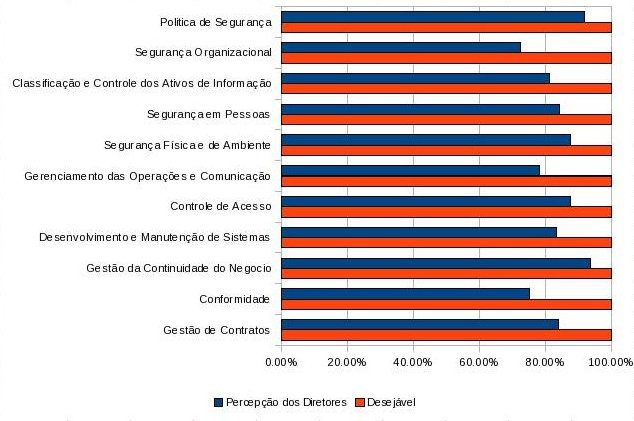
\includegraphics[height=\imgheight,width=\imgwidth]{graph_dir}
  \caption{Resultado {--} Percep��o dos Diretores}
  \label{img:graphdir}
\end{figure}

\begin{figure}[H]
  \centering
	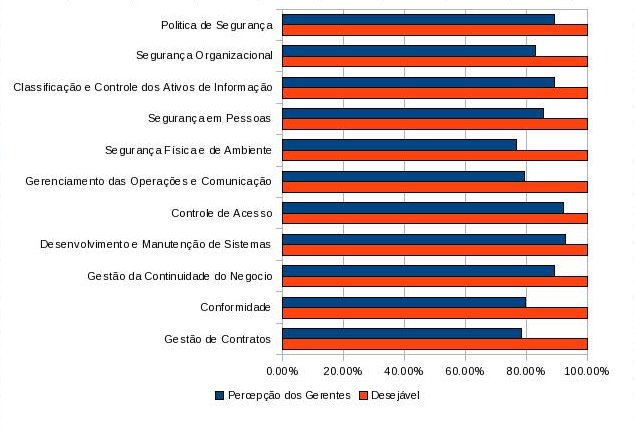
\includegraphics[height=\imgheight,width=\imgwidth]{graph_ger}
  \caption{Resultado {--} Percep��o dos Gerentes}
  \label{img:graphger}
\end{figure}

\begin{figure}[H]
  \centering
	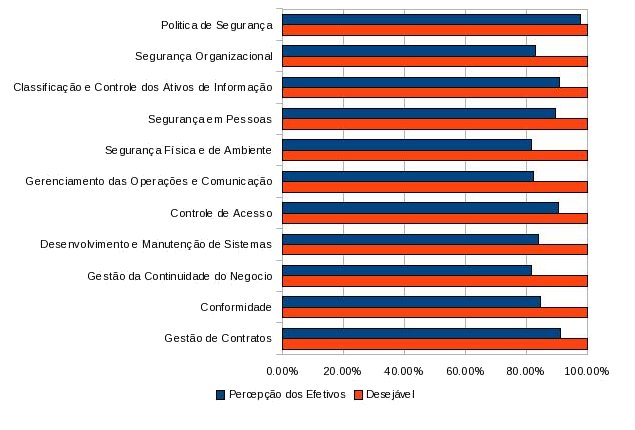
\includegraphics[height=\imgheight,width=\imgwidth]{graph_efe}
  \caption{Resultado {--} Percep��o dos Funcion�rios Efetivos}
  \label{img:graphefe}
\end{figure}

\begin{figure}[H]
  \centering
	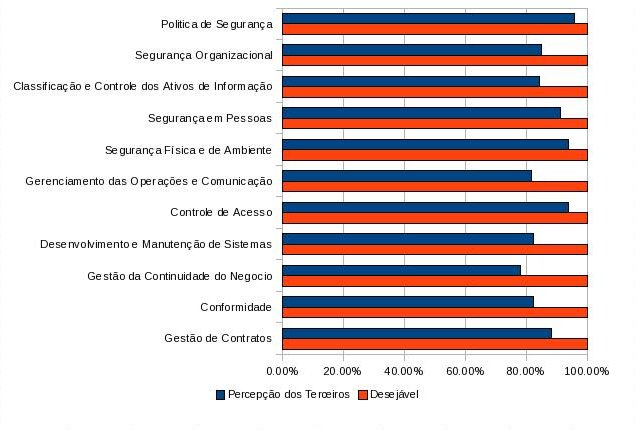
\includegraphics[height=\imgheight,width=\imgwidth]{graph_ter}
  \caption{Resultado {--} Percep��o dos Terceiros}
  \label{img:graphter}
\end{figure}

\begin{figure}[H]
  \centering
	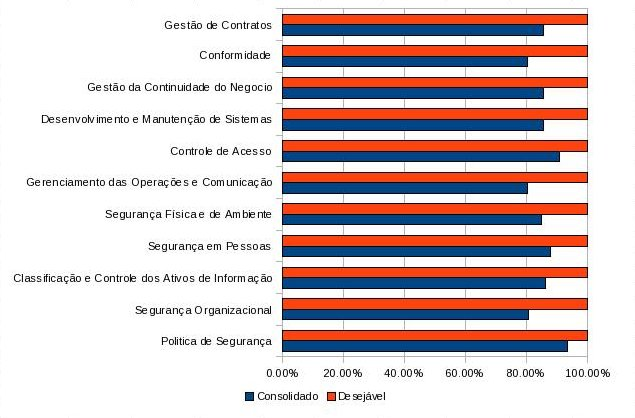
\includegraphics[height=\imgheight,width=\imgwidth]{graph_con}
  \caption{Resultado {--} Percep��es Consolidadas}
  \label{img:graphcon}
\end{figure}

\clearpage

